% =============================================================================
% MIN-REPORT-RL: A Minimum-Reportable-Stack Standard for
%                Reinforcement-Learning Post-Training of LLMs
% =============================================================================
% Pillar 4 of the ZVF Program. POSITION PAPER (NeurIPS/ICML Position Track +
% MLRC / ICLR Reproducibility Track).
%
% This is a standalone article-class draft backed by the program's canonical
% shared bibliography at platform_hybrid/paper/references.bib.
% =============================================================================

\documentclass[11pt]{article}

\usepackage[utf8]{inputenc}
\usepackage[T1]{fontenc}
\usepackage[margin=1in]{geometry}
\usepackage{hyperref}
\usepackage{url}
\usepackage{booktabs}
\usepackage{amsmath}
\usepackage{amssymb}
\usepackage{xcolor}
\usepackage{enumitem}
\usepackage{microtype}
\usepackage{graphicx} % for \resizebox on wide tables
\usepackage{listings} % for JSON schema listings
\usepackage{tikz}
\usetikzlibrary{shapes,arrows.meta,positioning,calc}
\usepackage[numbers,sort&compress]{natbib}
\lstset{basicstyle=\small\ttfamily,frame=single,columns=fullflexible,breaklines=true}

\newcommand{\zvf}{\textsc{Zvf}}
\newcommand{\gu}{\textsc{Gu}}
\newcommand{\minreport}{\textsc{Min-Report-RL}}
\newcommand{\grpoReg}{\textsc{GRPO-Reg}}

\title{\minreport{}: Reporting the Stack, Not the Label\\
\large A Community Minimum-Reportable-Stack Standard and
Reproducibility-Audit Protocol\\for Group-Relative RL Post-Training of LLMs}

\author{Arvind C R\thanks{Pillar~4 of the ZVF Program.}\\
PES University\\\texttt{arvindcr4@gmail.com}}

\date{\today}

\begin{document}
\maketitle

% ABSORBED → P05 (not an independent venue count)
\paragraph{Absorption (roster R06).}
This condensed community position is absorbed into
\texttt{paper\_P5\_minreport.tex} (MIN-REPORT-RL) and retires when P05 is
submitted. Do not count R06 as a separate venue paper.

% =============================================================================
\begin{abstract}
% =============================================================================
Reinforcement-learning post-training of large language models is reported as
though an algorithm label---PPO, GRPO, DPO, and the growing GRPO family
(DAPO, GSPO, Dr.GRPO, M-GRPO, GRESO, EDGE-GRPO, DARS, TreePo,
\ldots)---fixes the experiment. It does not.
In an audit of a group-relative RL runner, nominally identical visible
``GRPO'' configurations (same advertised model family, group size, learning rate, dataset,
seed, and step budget) produced last-10 training reward of $84.4\%$ on one
backend and $5.0\%$ on another---a $\sim 17\times$ gap~\citep{zvfaudit2026} with \emph{no visible
hyperparameter difference}. Provenance inspection later showed that the managed
stack also pinned a different base checkpoint. The $17\times$ number is therefore
an under-specification exhibit, not a backend causal estimate: the label was held
constant; the \emph{stack and model identity} were not. We argue that this
stack-conditioning is not an exotic edge case but the
default state of the field, and that the literature's current reporting norms
make it structurally impossible to tell whether a claimed algorithmic gain
survives a change of backend, sampler, reference-policy/KL handling, LoRA
configuration, or reward parser.

This position paper proposes \minreport{}: an eight-item
\emph{minimum-reportable-stack} checklist that every GRPO-family paper should
satisfy---seven run-manifest fields plus held-out pass@$k$ reporting---where
each item is included precisely because it is a documented
lever that can flip a head-to-head comparison. We then propose a concrete
reproducibility-audit protocol---re-implement DAPO, GSPO, Dr.GRPO, and AERO
inside one controlled language-model stack and report which claimed gains survive;
M-GRPO is assigned to a separate agentic stratum because its hierarchy is not a
minimal arithmetic-trainer hook. We specify the locked treatment matrix and
verdict rules without printing unexecuted result cells. We
close with an adoption path for getting TRL, verl, and OpenRLHF to log the
\minreport{} fields by default, and with responses to the obvious objections.
We do \emph{not} claim that any specific GRPO variant is overstated; we claim
that, under current reporting, the field cannot \emph{know}, and that this is
fixable with a few lines of telemetry.
\end{abstract}

\begin{figure}[htbp]
\centering
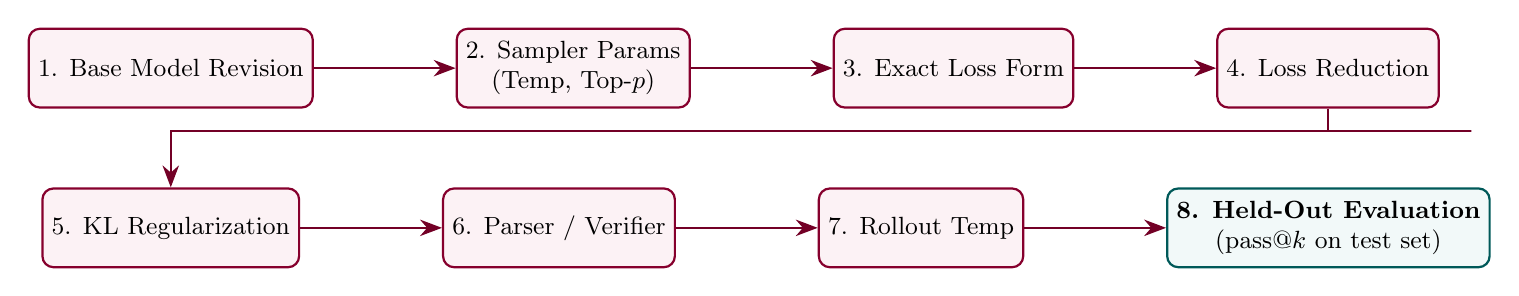
\begin{tikzpicture}[
    node distance=1.5cm and 1.8cm,
    box/.style={rectangle, draw=purple!70!black, fill=purple!5, thick, rounded corners, align=center, minimum height=1.0cm, minimum width=2.4cm, font=\small},
    evalbox/.style={rectangle, draw=teal!70!black, fill=teal!5, thick, rounded corners, align=center, minimum height=1.0cm, minimum width=3.2cm, font=\small},
    arrow/.style={-{Stealth[scale=1.2]}, thick, draw=purple!60!black}
]
    \node [box] (m) {1. Base Model Revision};
    \node [box, right=of m] (s) {2. Sampler Params\\(Temp, Top-$p$)};
    \node [box, right=of s] (l) {3. Exact Loss Form};
    \node [box, right=of l] (r) {4. Loss Reduction};

    \node [box, below=1.0cm of m] (k) {5. KL Regularization};
    \node [box, right=of k] (p) {6. Parser / Verifier};
    \node [box, right=of p] (t) {7. Rollout Temp};
    \node [evalbox, right=of t] (e) {\textbf{8. Held-Out Evaluation}\\($\text{pass}@k$ on test set)};

    \draw [arrow] (m) -- (s);
    \draw [arrow] (s) -- (l);
    \draw [arrow] (l) -- (r);
    \draw [arrow] (r) |- ($(r.east)+(0.4,-0.8)$) -| (k);
    \draw [arrow] (k) -- (p);
    \draw [arrow] (p) -- (t);
    \draw [arrow] (t) -- (e);
\end{tikzpicture}
\caption{\textbf{MIN-REPORT-RL Stack Contract Architecture (Pillar 4).} The eight required stack elements: seven run-manifest fields (1--7) plus held-out evaluation linkage (8), preventing unannounced stack shifts.}
\label{fig:min_report_architecture}
\end{figure}

% =============================================================================
\section{Introduction: The Telemetry and Reporting Gap}
\label{sec:intro}
% =============================================================================

\noindent\emph{Scope note (2026-07-11 canonicalization).} This document is
the condensed community-position statement of the \minreport{} standard.
The full-length treatment --- the measured exhibits, live-corpus coupling
analysis, threat model with flip-risk grades, toolchain, and verifier
implementation --- is the Pillar-5 paper \emph{``Report the Stack, Not the
Label: RL-for-LLM Results Are Stack-Conditioned''}
(\texttt{platform\_hybrid/paper/paper\_P5\_minreport}). The two documents
share the same eight-item standard; the Pillar-5 paper is canonical for
evidence, this one for the community-facing statement.

\begin{figure}[htbp]
\centering
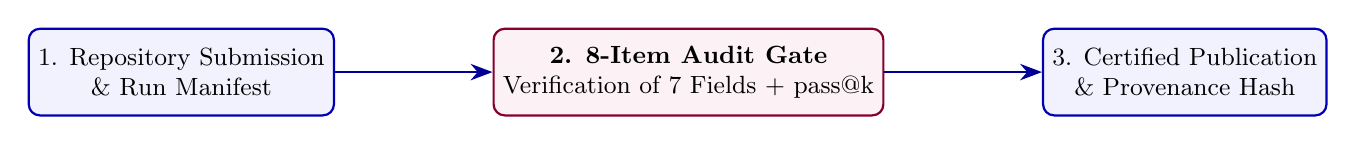
\begin{tikzpicture}[
    node distance=1.5cm and 2.0cm,
    stepbox/.style={rectangle, draw=blue!70!black, fill=blue!5, thick, rounded corners, align=center, minimum height=1.1cm, minimum width=3.2cm, font=\small},
    gatebox/.style={rectangle, draw=purple!70!black, fill=purple!5, thick, rounded corners, align=center, minimum height=1.1cm, minimum width=3.4cm, font=\small},
    arrow/.style={-{Stealth[scale=1.2]}, thick, draw=blue!60!black}
]
    \node [stepbox] (repo) {1. Repository Submission\\\& Run Manifest};
    \node [gatebox, right=of repo] (audit) {\textbf{2. 8-Item Audit Gate}\\Verification of 7 Fields + pass@k};
    \node [stepbox, right=of audit] (pub) {3. Certified Publication\\\& Provenance Hash};

    \draw [arrow] (repo) -- (audit);
    \draw [arrow] (audit) -- (pub);
\end{tikzpicture}
\caption{\textbf{Community Reproducibility Audit Lifecycle (R06).} Verifying stack compliance before accepting benchmark claims.}
\label{fig:min_report_lifecycle}
\end{figure}

A reader of the 2023--2026 RL-for-LLM literature could be forgiven for
believing that ``we trained with GRPO'' is a complete experimental
description. It is not. The same three-letter label is attached to runs that
differ in their loss form (is there a PPO ratio? a clip? a completion-only
token mask?), their reference-policy and KL handling (frozen reference? KL
penalty in the loss, or in the reward, or absent?), their sampler and backend
(vLLM vs.\ a managed inference API; bf16 vs.\ fp32 logits), their group-size
schedule, and the parser that converts a generation into a scalar reward. Each
of these is, individually, sufficient to move a result. Together they form a
\emph{treatment} that the algorithm label does not name.

This is the LLM-post-training analogue of the deep-RL reproducibility crisis
documented a decade ago \cite{henderson2018deep,islam2017reproducibility},
now recurring one abstraction level up. The earlier crisis was about code-level
and hyperparameter variance within a single algorithm; the present one is
worse, because the ``stack'' spans a managed API whose loss we cannot inspect,
a tokenizer and chat template that silently change the prompt, a sampler whose
numerics differ from the trainer's, and a reward parser that can reward a
format artifact instead of a correct answer.

\paragraph{The concrete trigger.}
In an audit of a critic-free group-relative runner \cite{zvfaudit2026}, we
attempted a deliberately boring comparison: hold the \emph{visible} GRPO
configuration fixed---Qwen3-8B-family, group size $G=8$, learning rate $10^{-5}$,
GSM8K, 30 steps, seed~42---and change the launch stack. A managed runner reached
$84.4\%$ last-10 training reward; TRL on an H100 reached $5.0\%$~\citep{zvfaudit2026}. No visible
hyperparameter explains the gap, and the managed run later proved to use a
different base checkpoint. What differs is everything the label omits:
checkpoint and tokenizer identity, prompt construction, sampler behavior, loss
masking, KL/reference handling, optimizer defaults, LoRA target modules,
precision, rollout plumbing, checkpoint selection, and the evaluator. The
comparison is not evidence that one backend is better; it is evidence that
``the GRPO config'' was \emph{under-specified}. If a nominal backend comparison can span a
$17\times$ result while also changing the
base checkpoint, then a head-to-head between
two GRPO \emph{variants}---each implemented in its own stack---tells us almost
nothing about the variants.

\paragraph{The family is growing faster than its reporting.}
The TMLR survey of agentic RL \cite{agenticrlsurvey2026} now catalogs, in a
single comparison table, more than twenty GRPO-family variants---and a
striking fraction of them (DAPO's dynamic sampling, GRESO's pre-rollout
filtering, EDGE-GRPO's \emph{advantage collapse} mitigation, DARS's
difficulty-aware reallocation) intervene on the same underlying lever: the
fraction of groups whose identical rewards contribute zero gradient, i.e.\
the quantity \zvf{} measures. Not one of the cataloged variant papers
reports a per-step dead-group trajectory or the stack fields below, so
their relative standings are, under current norms, unattributable. The
same survey's mechanistic synthesis supplies a second indictment of current
reporting: roughly two-thirds of the RL-for-reasoning studies it reviews
report only pass@1, although pass@$k$ curves are what distinguish a model
whose solution \emph{distribution was sharpened} from one whose solution
\emph{support expanded}. A variant can ``win'' at pass@1 by concentrating
probability on already-reachable solutions while strictly shrinking the
set of problems it can solve at pass@32. Under pass@1-only reporting, these
two outcomes---one an optimization of sampling, the other a capability
change---are indistinguishable. This motivates the eighth item of the
standard.

\paragraph{Why this is a reporting problem, not just a science problem.}
The gap above is not a bug to be fixed by a better trainer; it is information
that is routinely \emph{not logged}. Most papers do not report whether the KL
term was in the loss or the reward, whether the token mask was completion-only,
what the sampler precision was, or what the per-step group-size schedule looked
like. They also rarely report the per-step optimization telemetry---in our
framework, the Zero-Variance Fraction (\zvf{}) and Gradient Utilization
(\gu{})---that would reveal whether a run had any usable learning signal at all
\cite{zvfaudit2026}. A field cannot audit what it does not record. The fix is
cheap: a small, fixed set of fields, logged by default.

\paragraph{Scope and provenance of the worked numbers.}
The concrete numbers in this paper used as motivating examples
($84.4\%$/$\,5.0\%$/$\,17\times$ in the audit;
$61.6$--$89.6\%$ prompt-token loss magnitude;
$82.0\%\to83.3\%$ held-out control at $p=0.26$;
$95.0$--$98.1\%$/$\,95.0\%$ Llama-3.3-70B run)
are inherited from the audit paper that motivated this
position piece~\citep{zvfaudit2026}. A reader who wants to verify the numbers should consult that
paper; this manuscript presents them as illustrative of the
\emph{kind} of stack-driven flip, not as re-derivable from a fresh
run. The shared bibliography records the companion as a working paper until a
stable public identifier is assigned.
We do \emph{not} claim that any specific number here is independently
verifiable against the present manuscript's experimental record.

\paragraph{Contributions.}
This paper makes three:
\begin{enumerate}[leftmargin=1.6em, itemsep=2pt]
  \item \textbf{The stack-conditioning thesis, sharpened into a reporting
        standard.} We restate and extend the audit finding that algorithm
        labels are under-specified treatments (\S\ref{sec:stack}), and convert
        it into \minreport{}: an eight-item minimum-reportable-stack checklist
        in which every item is justified by a mechanism through which it can
        flip a comparison (\S\ref{sec:standard}).
  \item \textbf{A controlled reproducibility-audit protocol.} We specify a
        single-stack re-implementation of DAPO, GSPO, Dr.GRPO, and AERO,
        with a pre-registered analysis that reports which claimed gains survive
        when the stack is held fixed (\S\ref{sec:audit}); M-GRPO is evaluated
        separately in an agentic environment.
  \item \textbf{An adoption path.} We describe concrete, low-friction changes
        to TRL, verl, and OpenRLHF so that the \minreport{} fields are emitted
        by default, plus a venue checklist (\S\ref{sec:adoption}).
\end{enumerate}

% =============================================================================
\section{The Stack-Conditioning Problem}
\label{sec:stack}
% =============================================================================

\paragraph{Thesis.}
\emph{Algorithm rankings in RL post-training are stack-conditioned.} A claim of
the form ``method $A$ beats method $B$'' is, in current practice, a claim about
two \emph{full stacks} $S_A$ and $S_B$ that happen to be tagged $A$ and $B$. The
quantities that determine the outcome---backend and sampler numerics, the exact
loss form (ratio, clip, token mask), reference-policy and KL handling, LoRA
target modules and rank, precision, the reward parser, the group-size schedule,
checkpoint selection, and the evaluation harness---are co-determinants of the
result, and they are typically \emph{confounded with the label}. In a one-way
variance decomposition over a heterogeneous run corpus, the framework/library
factor and the training-algorithm factor each explain roughly half of the
variance in the outcome ($\eta^2 \approx 0.55$ for both), but these factors are
themselves confounded with model, backend, reward, hardware, and task
\cite{zvfaudit2026}. ``Algorithm'' and ``stack'' are not separable in the
existing literature because nobody reports the stack.

\paragraph{A comparison that flips.}
Consider the minimal worked example from the audit. The \emph{visible} GRPO
configuration is matched exactly:
\begin{center}
\small
\begin{tabular}{@{}lll@{}}
\toprule
\textbf{Visible config (held constant)} \& \textbf{Backend $S_1$} \& \textbf{Backend $S_2$}\\
\midrule
Advertised model family \& Qwen3-8B \& Qwen3-8B \\
Exact base checkpoint \& \multicolumn{2}{c}{not matched; recovered only after the run} \\
Group size $G$ \& 8 \& 8 \\
Learning rate \& $10^{-5}$ \& $10^{-5}$ \\
Dataset / split \& GSM8K-500 \& GSM8K-500 \\
Steps \& 30 \& 30 \\
Seed \& 42 \& 42 \\
\midrule
\textbf{Last-10 training reward} \& $\mathbf{84.4\%}$ \& $\mathbf{5.0\%}$ \\
\bottomrule
\end{tabular}
\end{center}
A na\"ive reader concludes ``$S_1$'s GRPO is $17\times$ better.'' The correct
reading is that the two rows are \emph{different treatments wearing the same
label}: the loss form, token mask, KL/reference handling, sampler precision,
LoRA targets, optimizer defaults, and reward parser were never held fixed
because they were never reported, hence never matched. Flip any one of them and
the ranking can invert. This is the entire problem in one table: the label is
constant, the conclusion is determined by the unreported stack.

\paragraph{Why the GRPO family makes this acute.}
The methods this paper targets---DAPO, GSPO, Dr.GRPO, M-GRPO, and the broader
variance-mitigation line (AERO, CPPO, NGRPO, Scaf-GRPO)
\cite{yu2025dapo,qwen2025gspo,tong2025drgrpo,hong2025mgrpo,zhang2026aero,
lin2025cppo,nan2025ngrpo,zhang2025scaffgrpo}---are typically defined as
\emph{small deltas} on a
base GRPO loop: a changed advantage normalization, a clip-bound tweak, a token
mask, a length penalty, an exploration bonus, an adaptive group size. The size
of the claimed improvement is frequently \emph{smaller} than the stack effect
demonstrated above. When the treatment effect you are trying to measure is
$2$--$5$ points and the nuisance effect of an unreported stack difference is
tens of points, an uncontrolled head-to-head is not measuring the method. The
GRPO family is exactly the regime in which stack-conditioning is most likely to
masquerade as algorithmic progress.

% =============================================================================
\section{The \minreport{} Standard}
\label{sec:standard}
% =============================================================================

\minreport{} is a minimum-reportable-stack: the smallest set of fields such
that, if two GRPO-family papers both report them, a reader can tell whether
their comparison is confounded. Each item below is included \emph{because there
is a known mechanism by which it can flip a comparison}; an item that could not
change a ranking would not earn its place on a minimum list.

\paragraph{1. Loss form.}
\emph{Report:} whether the update uses a PPO-style importance ratio
$w_{i,t}=\pi_\theta/\pi_{\theta_{\text{old}}}$; whether and how it is clipped
(and the clip bounds, including asymmetric DAPO-style ``clip-higher'');
whether the token mask is completion-only or whole-sequence; and whether
advantages are normalized per-group, per-batch, or with a running estimate.
\emph{Why it can flip:} the choice of token mask changes the
\emph{objective}. In one diagnostic, $61.6$--$89.6\%$ of the full-sequence
\emph{loss magnitude} (raw NLL composition) came from \emph{prompt} tokens
rather than completion tokens \cite{zvfaudit2026}; a whole-sequence mask and
a completion-only mask are therefore different objectives sharing a name.
(Caveat, added 2026-07-11: under exactly group-centered advantages the
prompt-token \emph{gradient} contributions cancel within each group, so this
figure quantifies objective composition, not gradient leakage --- a
distinction that is itself rarely reported.) Dr.GRPO's contribution is
precisely a change to length/normalization in the loss \cite{tong2025drgrpo}; GSPO
changes the importance-sampling granularity \cite{qwen2025gspo}. If the baseline's
loss form is unreported, the variant's gain is unattributable. The stake is not
hypothetical: in our own companion panel, a documented-but-unwired loss flag
left six ``GRPO vs.\ Dr.GRPO'' arms silently training the identical objective,
and no reward, length, or ZVF trace revealed it --- only reading the runner
did. Loss form must be \emph{reported and verified}, not inferred from
plausible-looking outputs.

\paragraph{2. Reference policy and KL handling.}
\emph{Report:} whether a frozen reference policy is retained; whether the KL
term sits in the \emph{loss} or is folded into the \emph{reward}; the KL
coefficient and its schedule; and whether KL is estimated forward or reverse,
per-token or per-sequence. \emph{Why it can flip:} KL placement changes the
effective objective and the steady-state exploration. A runner that drops the
reference policy entirely (one optimizer step per rollout, no frozen reference)
is not doing the same thing as a KL-regularized GRPO, even at matched learning
rate \cite{zvfaudit2026}. Methods that add a second anchor (for example, an
additional KL or SFT-reference term) change steady-state \zvf{} and must be
recalibrated, not compared blind. The anchor, placement, and coefficient must
therefore be reported explicitly.

\paragraph{3. Sampler, backend, and precision.}
\emph{Report:} the rollout engine (vLLM, SGLang, a managed API, the trainer's
own \texttt{generate}; decoding parameters (temperature, top-$p$,
\texttt{max\_tokens}; logit precision in the sampler vs.\ the trainer (bf16 /
fp16 / fp32); and whether sampler and trainer share the same tokenizer and chat
template. \emph{Why it can flip:} the sampler defines the rollout distribution
that the group-relative update consumes. A managed, closed-source runner and an
open vLLM path can yield order-of-magnitude different training-reward
trajectories under similar visible configs. In our $17\times$ exhibit the
backend, sampler, and base checkpoint co-varied, so the exhibit motivates
reporting but does not identify a backend mechanism. Sampler precision can shift the probability
of mixed-reward groups, and hence the available gradient.

\paragraph{4. Per-step \zvf{} and \gu{} trajectory.}
\emph{Report:} the per-step Zero-Variance Fraction \zvf{} (fraction of prompts
whose $G$ completions all receive identical reward, contributing zero gradient)
and Gradient Utilization $\gu{}=1-\zvf{}$, logged for every training step.
\emph{Why it can flip:} \zvf{}/\gu{} is the telemetry that reveals \emph{whether
a run had any learning signal at all}. The mixed-group probability
$P(\text{usable}) \approx \frac{1}{N}\sum_x\!\left[1-(1-p_x)^G-p_x^G\right]$
shows that a group-relative update only has signal when sampled groups contain
reward diversity \cite{zvfaudit2026}. A method can ``win'' a comparison purely
because its stack happened to produce lower \zvf{} (more usable groups), not
because its algorithmic idea is better. Without the \zvf{}/\gu{} trajectory, a
collapsed run and a saturated run are indistinguishable from their final reward.
A fixed first-five-step rule (\zvf{}$\,\ge 80\%$ with reward $\le 5\%$) is a
cheap collapse triage; reporting the trajectory lets a reader apply it.

\paragraph{5. Group-size schedule (fixed or adaptive).}
\emph{Report:} the group size $G$ at every step, and the rule that changes it
if it is adaptive (e.g.\ AERO-style doubling/halving on a rolling \zvf{}
estimate). \emph{Why it can flip:} $G$ directly controls the mixed-group
probability above and is one of the strongest single knobs we measured---an
ablation on Qwen3-8B/GSM8K moved last-10 reward across a wide band as $G$ went
$2\!\to\!4\!\to\!8\!\to\!16$ \cite{zvfaudit2026}. An adaptive-$G$ method (AERO)
compared against a fixed-$G$ baseline is partly being credited for spending
more compute on hard prompts, an effect that must be separated from the
algorithmic claim \cite{zhang2026aero}.

\paragraph{6. Held-out split distinct from the reward environment.}
\emph{Report:} a held-out evaluation slice that is \emph{disjoint} from the
training prompts and scored by a harness, with sample size and a confidence
interval, reported \emph{separately} from online training reward. \emph{Why it
can flip:} online training reward is dynamics evidence, not capability
evidence. In the audit, a clean paired control improved only $82.0\%\to83.3\%$
($p=0.26$)~\citep{zvfaudit2026} on held-out GSM8K despite training reward near saturation; and
selecting checkpoints by training reward produced an $87$--$95\%$ ``capability''
band that is a selection artifact, not a causal lift \cite{zvfaudit2026}. A
variant that reports only training reward can show a large apparent gain that
vanishes held-out. Four Llama-3.3-70B seeds ranged $95.0$--$98.1\%$ on training
last-10 yet all landed on $95.0\%$ held-out~\citep{zvfaudit2026}---last-10 variance was
sampling noise, not generalization.

\paragraph{7. Decontamination probe results.}
\emph{Report:} the outcome of an explicit train/test contamination check
(n-gram or embedding overlap between training prompts and the held-out /
benchmark slice), and the parser's behavior on adversarial format-only inputs.
\emph{Why it can flip:} verifiable rewards do not eliminate reward hacking;
parser artifacts, format shortcuts, length effects, and train-prompt overfitting
can all inflate a reward without capability gain \cite{zvfaudit2026}. If the
benchmark slice overlaps the reward environment, a ``gain'' may be memorization;
if the parser rewards a format token, a ``gain'' may be a shortcut. A
contamination/parser probe is the minimum evidence that the reported number
measures the thing it claims to measure.

\paragraph{8. Pass@$k$ curves alongside pass@1.}
\emph{Report:} held-out pass@$k$ at $k \in \{1, 8, 32\}$ (or a stated
subset with justification), with the sampling temperature and completion
budget used for the estimate. \emph{Why it can flip:} pass@1 conflates two
different improvements---sharpening the output distribution over solutions
the base model could already reach, and expanding the set of reachable
solutions. The agentic-RL survey's synthesis \cite{agenticrlsurvey2026}
finds that roughly two-thirds of RL-for-reasoning papers report only
pass@1, while the studies that do report pass@$k$ frontiers repeatedly find
base models matching or overtaking their RL-tuned counterparts at large
$k$---i.e., the ``gain'' was distribution sharpening. A GRPO-variant
comparison scored at pass@1 alone can therefore rank the method that
sharpens above the method that generalizes, and the ranking can invert at
$k=32$. Because group-relative training acts directly on the sampling
distribution, this is not an exotic failure mode for the GRPO family; it is
the expected one.

\paragraph{Summary table.}
Table~\ref{tab:checklist} collects the standard. The companion
\texttt{CHECKLIST.md} provides a fillable appendix template.

\begin{table}[t]
\centering
\caption{The \minreport{} minimum-reportable-stack. Each item is on the list
because it is a documented lever that can flip a head-to-head comparison.}
\label{tab:checklist}
\small
\begin{tabular}{@{}rp{0.30\linewidth}p{0.50\linewidth}@{}}
\toprule
\# \& \textbf{Field} \& \textbf{Flip mechanism (why it is mandatory)}\\
\midrule
1 \& Loss form (ratio / clip / token mask / advantage norm.) \& Token mask reassigns gradient across prompt vs.\ completion tokens; clip and norm.\ are the actual variant deltas.\\
2 \& Reference policy + KL handling \& KL placement (loss vs.\ reward) and a frozen-vs-absent reference change the objective and exploration.\\
3 \& Sampler / backend / precision \& The sampler defines the rollout distribution; these fields co-varied with checkpoint identity in the $17\times$ under-specification exhibit~\citep{zvfaudit2026}.\\
4 \& Per-step \zvf{} / \gu{} trajectory \& Reveals whether the run had usable learning signal; separates collapse from saturation.\\
5 \& Group-size schedule (fixed / adaptive) \& $G$ sets the mixed-group probability; adaptive-$G$ confounds compute with algorithm.\\
6 \& Held-out split $\neq$ reward environment \& Training reward is not capability; selection-by-reward inflates apparent gains.\\
7 \& Decontamination probe results \& Verifiable rewards still admit parser/format/length/overlap hacking.\\
8 \& Pass@$k$ curves alongside pass@1 \& Pass@1-only scoring cannot distinguish distribution sharpening from capability gain; rankings can invert at large $k$.\\
\bottomrule
\end{tabular}
\end{table}

\subsection{Measured stack effects (new evidence, 2026-07)}
\label{sec:measured}

Three of the standard's items now carry \emph{quantified} first-party
evidence from the companion experiments suite
(\texttt{zvf-program/experiments-next/results/}), replacing argument by
anecdote.

\paragraph{Item 3, measured: the sampler moves frontier metrics.}
Holding model, prompts (200 GSM8K test problems), temperature, seed, and
parser byte-identical, and swapping \emph{only} the sampling backend:
\begin{center}
\begin{tabular}{@{}lccc@{}}
\toprule
Backend \& pass@1 \& pass@8 \& pass@32 \\
\midrule
Managed (Tinker) sampler \& 30.4\% \& 79.7\% \& 91.0\% \\
vLLM 0.24 on A100 \& 30.6\% \& 77.8\% \& 89.0\% \\
\bottomrule
\end{tabular}
\end{center}
Point estimates are backend-robust ($+0.2$ at pass@1) while the pass@32
frontier shifts by $2.0$ points and individual problems move by up to
$|11|/32$ solutions. Any cross-paper comparison of frontier metrics that
does not report the sampler is therefore confounded at the
$\sim$2-point scale --- the same scale as many claimed algorithmic gains.

\paragraph{Item 1, measured: silent export/loader incompatibilities.}
Evaluating LoRA adapters trained on a managed stack inside an open
inference stack required reverse-engineering two undocumented format
deltas: \texttt{target\_modules="all-linear"} (PEFT shorthand the open
loader rejects) and the unembedding trained under
\texttt{model.unembed\_tokens} (the open loader accepts only
\texttt{lm\_head}). Without remapping, \emph{every} cross-stack evaluation
of these 21 public adapters fails --- loudly in our harness, but a wrapper
that silently skipped the adapter would have produced base-model numbers
labeled as post-RL results. This is precisely the class of confound item 1
exists to surface.

\paragraph{Item 8, exemplified: the panel pass@1 alone would misreport.}
A matched base-vs-post-RL panel (four adapters trained at
$G\in\{2,4,16,32\}$; one stack; same problems) shows pass@1 deltas
scattered from $-0.5$ to $+1.9$ points --- under pass@1-only reporting,
the $G{=}2$ arm would be called a \emph{regression}. The pass@32 frontier
tells the opposite, consistent story: all four arms improve by $+1.5$ to
$+2.5$ points. Neither reading reaches significance at a single training
seed (the deltas sit within the measured sampler and eval-seed noise
bands above), which is itself the point: \textbf{without pass@$k$ curves
and stated noise bands, this panel supports any narrative a reader
prefers.} With them, it supports exactly one claim: a small,
directionally consistent frontier shift requiring multi-seed replication.

% =============================================================================
\section{Proposed Reproducibility Audit}
\label{sec:audit}
% =============================================================================

The \minreport{} standard tells authors what to report. The audit tells the
community what to \emph{check}: \emph{which claimed GRPO-family gains survive
when the stack is held fixed?}

\paragraph{Design.}
Re-implement four prominent minimal-delta variants---DAPO, GSPO, Dr.GRPO, and
AERO \cite{yu2025dapo,qwen2025gspo,tong2025drgrpo,zhang2026aero}---as
\emph{declared overrides on a single shared trainer}. M-GRPO
\cite{hong2025mgrpo} changes planner/sub-agent credit and is audited in a
separate agentic stratum. Everything
in the \minreport{} list except the variant's defining delta is held identical
across arms: the same base checkpoint and tokenizer, the same vLLM sampler and
precision, the same reference-policy/KL handling, the same LoRA targets and
rank, the same optimizer, the same reward parser, the same group-size schedule
(where the variant does not itself change it), the same held-out slice, and the
same evaluation harness and seed sweep. Only the named hook differs (loss form,
advantage normalization, clip rule, masking, or group-sizing). This is the same
methodology already validated for the variance-mitigation head-to-head, where
AERO/CPPO/NGRPO/Scaf-GRPO were each implemented as one hook on a shared GRPO
trainer with tokenizer, sampler, optimizer, LoRA adapters, evaluation harness,
and seed sweep held identical \cite{zvfaudit2026}.

\paragraph{Two readings per variant.}
For each variant we report (i) its result \emph{as published} (its own stack,
its own numbers) and (ii) its result \emph{in the controlled stack}. The
quantity of interest is the \emph{survival} of the claimed gain: the
controlled-stack delta relative to the shared GRPO baseline, with a confidence
interval and a survival verdict (survives / shrinks / disappears / reverses).

\paragraph{Pre-registration.}
The arm list, the shared stack specification, the held-out slice, the seed set,
and the survival thresholds are fixed before any controlled run is scored, to
avoid the selection-by-reward over-optimism the audit itself warns against
\cite{zvfaudit2026}. Every arm reports the full \minreport{} block.

\paragraph{Locked audit matrix.}
The position paper does not print empty result tables. It locks the treatment
matrix in Table~\ref{tab:audit-protocol}; the companion audit generates result
and telemetry tables only after every preregistered arm is complete.

\begin{table}[t]
\centering
\caption{\textbf{Preregistered single-stack treatment matrix.} The first five
rows share one language-model trainer. M-GRPO changes the environment and credit
structure, so it is a separate agentic stratum rather than a misleading
``minimal hook'' in the arithmetic audit.}
\label{tab:audit-protocol}
\small
\begin{tabular}{@{}lp{0.42\linewidth}p{0.28\linewidth}@{}}
\toprule
\textbf{Arm} \& \textbf{Only permitted treatment change} \& \textbf{Group schedule}\\
\midrule
GRPO \& none (reference arm) \& fixed $G=8$\\
DAPO \& asymmetric clip plus dynamic resampling \& reported realized $G$/rollouts\\
GSPO \& sequence-level rather than token-level IS ratio \& fixed $G=8$\\
Dr.GRPO \& remove within-group standard-deviation normalization \& fixed $G=8$\\
AERO \& adaptive rollout allocation, selective rejection, posterior state \& full schedule reported\\
M-GRPO \& hierarchical planner/sub-agent credit assignment \& separate agentic stratum\\
\bottomrule
\end{tabular}
\end{table}

\paragraph{Preregistered statistical protocol.}
The independent unit is a seed, not a per-step reward. The full audit uses
eight seeds $\{11,23,37,53,71,89,107,131\}$ per core arm and a fixed held-out
set of 500 prompts. The primary estimand is the paired seed-level held-out
delta relative to GRPO at the fixed final checkpoint; training last-10 reward,
\zvf{}/\gu{}, collapse rate, realized rollouts, and wall-clock time are
secondary. We report a paired bootstrap 95\% CI and Benjamini--Hochberg-adjusted
tests over the four core comparisons.

Let $r=\Delta_{\mathrm{controlled}}/\Delta_{\mathrm{published}}$ only when
model, task, split, and metric are compatible. A variant \emph{retains} its
published effect if the controlled 95\% CI excludes zero and its lower bound
implies $r\ge0.5$. It \emph{survives} if that CI excludes zero but no compatible
published delta exists or the half-gain rule fails; it \emph{reverses} if the
upper CI is below zero; otherwise it is \emph{inconclusive}.
``Disappears'' requires an equivalence test whose entire 90\% CI lies inside
$[-m,m]$ for the locked absolute held-out margin $m=0.01$. Before scoring,
the analysis reports the seed-level standard deviation and achieved minimum
detectable effect; if the MDE exceeds $m$, disappearance is unavailable and the
verdict remains inconclusive. These rules are mirrored in the machine-readable
preregistration beside the companion audit.

\paragraph{Honest scoping.}
The audit's deliverable is \emph{not} ``method $X$ is fake.'' It is a survival
map: for each variant, the fraction of its claimed gain that persists when the
stack is the same. Some gains will survive (they are real algorithmic
contributions); some will shrink (they were partly stack); some may disappear
(they were stack). All three outcomes are informative, and reporting them is
the contribution.

% =============================================================================
\section{Adoption Path}
\label{sec:adoption}
% =============================================================================

A standard nobody can comply with cheaply will not be adopted. \minreport{} is
designed so that the marginal cost to an author is close to zero \emph{if the
trainers log it by default}.

\paragraph{Make the trainers emit it.}
The seven run-manifest fields are already computable inside every major open
trainer; pass@k is a post-training evaluation artifact. The marginal work is
to write the manifest once, in a stable schema, to compute
\zvf{}/\gu{} from the grouped reward tensor that GRPO already materializes.

\subparagraph{A concrete TRL plugin proposal: \texttt{trl-min-report-rl}.}
We specify a small TRL extension that would make adoption automatic. For every
\texttt{GRPOTrainer.train()} call it would emit a run-start JSON block
containing the seven manifest fields, then log per-step \zvf{}/\gu{} from the
actual grouped rewards used by GRPO. This package is not yet released; its
proposed shape is:
\begin{verbatim}
trl_min_report_rl/
  __init__.py
  config.py              # MinReportRLConfig dataclass + CLI flags
  callback.py            # run-start manifest + finalization
  grpo_mixin.py          # reward-tensor hook
  emitter.py             # JSONL + stdout + logger adapters
  schema/
    grpo_run_start.v0.1.json
    grpo_step.v0.1.json
\end{verbatim}
The public API is a single extra argument to \texttt{GRPOConfig}:
\begin{verbatim}
args = GRPOConfig(..., report_min_report_rl=True)
trainer = MinReportGRPOTrainer(
    model=model, args=args, reward_funcs=[reward_fn],
    train_dataset=train_ds, eval_dataset=heldout_ds,
    processing_class=tokenizer, min_report_rl=MinReportRLConfig(...))
\end{verbatim}
A no-subclass adapter, \texttt{enable\_min\_report\_rl(trainer, config)}, is a
proposed compatibility surface for existing code.

The critical hook is \texttt{on\_grpo\_rewards\_computed}, called after reward
functions return and after distributed gather, but before advantage
normalization. It receives \texttt{rewards\_per\_func}, \texttt{reward\_weights},
and \texttt{num\_generations}, and computes
\[
\text{ZVF}_t = \frac{1}{N}\sum_{x=1}^{N}
  \mathbf{1}\big[\operatorname{Var}(r_{x,1},\dots,r_{x,G})=0\big],
\qquad
\text{GU}_t = 1 - \text{ZVF}_t,
\]
where unusable (all-NaN) groups are counted as zero-variance. The hook logs both
human-readable scalars (\texttt{min\_report\_rl/zvf},
\texttt{min\_report\_rl/gu}, \texttt{min\_report\_rl/usable\_groups}) and a
per-step JSON event.

\subparagraph{Upstream surface.}
The cleanest upstream TRL change adds three elements to \texttt{GRPOConfig}:
\texttt{report\_min\_report\_rl}, \texttt{min\_report\_rl\_strict}, and
\texttt{min\_report\_rl\_output\_dir}; plus two trainer methods
(\texttt{\_emit\_min\_report\_rl\_run\_start} and
\texttt{\_emit\_min\_report\_rl\_step}) and the reward-path hook call. That
is the ``few lines of telemetry'' version of the standard.

\subparagraph{Run-start manifest.}
The first line of \texttt{min\_report\_rl.jsonl} is a JSON object whose
\texttt{min\_reportable\_stack} field contains the seven run-manifest items.
The eighth standard item, pass@k alongside pass@1, belongs in the evaluation
report. A manifest fragment is
shown in Listing~\ref{lst:runstart}; the full schema is in the
\grpoReg{} catalog paper \cite{grpoRegistry2026}.

\begin{lstlisting}[caption={Fragment of the
  \texttt{min\_report\_rl} run-start manifest.}, label={lst:runstart}]
{
  "event": "min_report_rl.run_start",
  "min_reportable_stack": {
    "1_loss_form": {"status":"known", "loss_type":"dapo", ...},
    "2_reference_policy_kl": {"status":"known", "kl": {"enabled":false}},
    "3_sampler_backend_precision": {"rollout_engine":"vllm", ...},
    "4_zvf_gu_trajectory": {"enabled":true, "basis":"weighted_reward", ...},
    "5_group_size_schedule": {"train_num_generations":8, ...},
    "6_heldout_split": {"heldout_dataset_id":"gsm8k:test:500", ...},
    "7_decontamination_probes": {"ngram_overlap":{"passed":true}, ...}
  }
}
\end{lstlisting}

\subparagraph{Other trainers.}
verl's actor/rollout separation makes sampler, precision, and group-size
schedule first-class; OpenRLHF's reference-model and KL options map directly
onto item~2. Both can emit the same manifest block and per-step telemetry using
the same shared emitter. The schema is trainer-agnostic; only the source of each
field changes.

\paragraph{Enforcement and audit tooling.}
The same manifests feed the implemented
\path{platform_hybrid/registry/query.py stackdiff} command
(\S\ref{sec:tooling}), which compares registry entries and flags label-flip
risk. The implemented \path{registry/provenance/minreport.py verify} command
grades generated provenance records. A future literature-scale Auditor would
score an existing paper or repo against the eight-item checklist,
assigns a 0--100 reproducibility-auditable badge, and produces a reviewer-facing
summary \cite{zvfaudit2026}. The audit paper's locked aggregator turns the
controlled single-stack audit of \S\ref{sec:audit} into a fail-closed result
validator. A full launcher would lock the shared stack, expand each variant as
a declared hook, and compute verdicts from paired seed-level held-out deltas
\cite{zvfaudit2026}. Together these tools turn the abstract standard into a
mechanical check that venues and reviewers can run in CI.

\paragraph{Make the venues ask for it.}
Add a \minreport{} block to the reproducibility checklist for the RL-for-LLM
track, analogous to the existing NeurIPS/ICML reproducibility checklists. The
companion \texttt{CHECKLIST.md} is written to be dropped verbatim into a paper's
appendix.

\paragraph{Make it auditable post hoc.}
For already-published work, the same JSON block can be reconstructed from
release artifacts where they exist. The audit of \S\ref{sec:audit} doubles as a
demonstration: it re-derives the \minreport{} block for the controlled arms and shows
the format is sufficient to detect confounded comparisons.

% =============================================================================
\section{Objections and Responses}
\label{sec:objections}
% =============================================================================

\paragraph{``This is just `report your hyperparameters.'\,''}
No. Hyperparameter tables already exist and the $17\times$ gap~\citep{zvfaudit2026} occurred
despite similar visible recipes because checkpoint and stack identity were not
actually matched. \minreport{} names the fields
that hyperparameter tables systematically omit---loss form, KL placement,
sampler precision, per-step \zvf{}/\gu{}, group-size schedule, held-out
disjointness, contamination probe---precisely because each is a demonstrated
flip lever, not a tuning knob.

\paragraph{``Eight items is too many / too few.''}
Each item earns its place by a flip mechanism (\S\ref{sec:standard}); removing
any one reopens a known confound. The list is a \emph{minimum}, not a maximum:
authors may report more. We deliberately stop at eight because that is the set
that, in our audit and in the survey-documented pass@$k$ reporting gap
\cite{agenticrlsurvey2026}, was sufficient to explain the comparisons that
flipped.
If the audit surfaces a ninth recurring confound, the versioned standard will
extend the list only with an explicit flip mechanism and migration note.

\paragraph{``Re-implementations are unfaithful, so the audit is unfair.''}
The audit reports \emph{both} readings (published and controlled) and frames the
result as survival, not refutation. An unfaithful re-implementation is itself a
finding: if a variant's gain depends on an unstated stack detail that a careful
re-implementer cannot reproduce from the paper, that is a reporting failure the
standard is designed to surface. We will publish every arm's full \minreport{}
block so disagreements are about specific fields, not vibes.

\paragraph{``Closed/managed backends can't comply.''}
Partly true, and that is the point: a closed runner cannot expose its loss form
or KL handling, so results from it should be scoped as ``this platform's
implementation,'' not ``GRPO'' \cite{zvfaudit2026}. The standard makes that
scoping explicit rather than letting a closed-stack number stand in for an
algorithm.

\paragraph{``\zvf{}/\gu{} is your own metric; why mandate it?''}
\zvf{}/\gu{} is one cheap instantiation of a necessary quantity---\emph{did the
run have usable group-relative signal?}---and we accept substitutes. Under
dense process rewards or scaffolded exploration, \zvf{} degenerates and should
be replaced by per-step reward variance or a gradient-norm-variance surrogate
\cite{zvfaudit2026}. Item~4 mandates \emph{a usable-signal trajectory}, of which
\zvf{}/\gu{} is the default; the point is that \emph{some} such telemetry must be
reported.

% =============================================================================
\section{Companion Tooling: \texttt{grpo-stackdiff}}
\label{sec:tooling}
% =============================================================================

A standard is easier to adopt if reviewers can check it mechanically. The
current reference command,
\path{python3 platform_hybrid/registry/query.py stackdiff <entry-a> <entry-b>},
consumes two registry records and reports R0--R5 label-flip risk. We also sketch
a richer version that would consume arbitrary \minreport{} manifests and use
the L0--L7 taxonomy below. Neither command is a replacement for the audit of
\S\ref{sec:audit}; it is an enforcement layer that tells a reviewer, in
seconds, whether a head-to-head is stack-comparable.

\paragraph{Manifest contract.} Each run is a YAML/JSON block containing the
eight \minreport{} fields, plus run identity (trainer, version, seed, hardware),
model and tokenizer hashes, LoRA configuration, optimizer settings, and results.
The schema is the JSON block proposed in \S\ref{sec:adoption}.

\paragraph{Diff taxonomy.} Every field difference receives three labels:
\begin{itemize}[leftmargin=1.4em, itemsep=2pt]
  \item \textbf{Lever.} One of eight lever groups: L0~run identity/provenance,
    L1~loss form, L2~reference policy and KL handling, L3~sampler/backend/
    precision, L4~usable-signal telemetry (\zvf/\gu{}), L5~group-size
    schedule, L6~held-out evaluation and checkpoint selection, L7~decontamination
    and parser robustness.
  \item \textbf{Diff kind.} EQUAL, COSMETIC, PROVENANCE, PARAMETRIC, SCHEDULE,
    SEMANTIC\_OBJECTIVE, DISTRIBUTIONAL, TELEMETRY, MISSING, OPAQUE, DERIVED, or
    INVALID\_TARGET.
  \item \textbf{Role.} TREATMENT\_DELTA if the user declares it as the
    algorithmic delta being tested; NUISANCE\_DELTA if it is an uncontrolled
    stack difference; COVERAGE\_GAP if the field is missing; INVALIDATOR if the
    comparison target is not common.
\end{itemize}

\paragraph{Flip-risk classes.} The tool compares each nuisance difference to
the reported comparison margin and classifies the overall risk as one of:
\begin{center}
\small
\begin{tabular}{@{}ll@{}}
\toprule
\textbf{Class} \& \textbf{Meaning}\\
\midrule
R0 \texttt{same} \& No meaningful difference.\\
R1 \texttt{cosmetic} \& Version string or comment only.\\
R2 \texttt{small} \& Estimated effect $<25\%$ of the comparison margin.\\
R3 \texttt{material} \& Effect $25$--$100\%$ of the margin; can shrink a claim.\\
R4 \texttt{flip\_capable} \& Effect bound $\	ext{\textgreater=}$ margin; can flip the ranking.\\
R5 \texttt{invalidating} \& The comparison target is not common.\\
RU \texttt{unknown} \& Missing or opaque evidence; comparison unverifiable.\\
\bottomrule
\end{tabular}
\end{center}

\paragraph{Verdict and CI integration.} The tool emits a deterministic verdict
(\texttt{STACK\_MATCHED}, \texttt{STACK\_MATERIAL}, \texttt{STACK\_CONFOUNDED},
\texttt{UNVERIFIABLE}, or \texttt{INVALID\_COMPARISON}) and an exit code, so a
paper's reproducibility workflow can fail a comparison that is
flip-capable. Example:
\begin{verbatim}
python3 platform_hybrid/registry/query.py stackdiff \
  colab-open_dapo_e3 tinker_dapo_qwen3.5-4b_gsm8k
\end{verbatim}

\paragraph{Role in the \minreport{} ecosystem.} Authors emit the JSON block;
venues ask for it; reviewers run the reference stackdiff command. The cost to an author
is still a few lines of telemetry; the cost to a reviewer is one command. The
tool turns the abstract stack-conditioning thesis of \S\ref{sec:stack} into a
concrete, reproducible check.

% =============================================================================
\section{Conclusion}
\label{sec:conclusion}
% =============================================================================

The RL-for-LLM literature is in a position the deep-RL community has seen
before: a three-letter label is doing the work of a full experimental
specification, and the unreported remainder of the stack can move a result by
more than the algorithmic effect anyone is trying to claim. We have argued that
this stack-conditioning is the default, demonstrated it with an under-specified
same-label comparison that differs by $17\times$, and proposed two coupled remedies: an
eight-item minimum-reportable standard (\minreport{}): seven manifest fields
that expose known confounds plus a pass@k evaluation artifact, and a controlled
single-stack audit of DAPO, GSPO,
Dr.GRPO, and M-GRPO that reports which claimed gains survive. Neither remedy
requires new science---only a few fields of telemetry and the discipline to log
them. The cost is a JSON block; the payoff is a literature whose comparisons one
can actually trust.

\bibliographystyle{plainnat}
\bibliography{../../platform_hybrid/paper/references}



\begin{figure}[htbp]
\centering
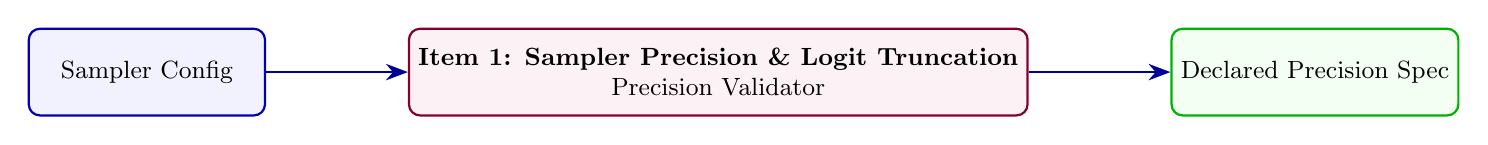
\begin{tikzpicture}[
    node distance=1.4cm and 1.8cm,
    box1/.style={rectangle, draw=blue!70!black, fill=blue!5, thick, rounded corners, align=center, minimum height=1.1cm, minimum width=3.0cm, font=\small},
    box2/.style={rectangle, draw=purple!70!black, fill=purple!5, thick, rounded corners, align=center, minimum height=1.1cm, minimum width=3.4cm, font=\small},
    box3/.style={rectangle, draw=green!70!black, fill=green!5, thick, rounded corners, align=center, minimum height=1.1cm, minimum width=3.2cm, font=\small},
    arrow/.style={-{Stealth[scale=1.2]}, thick, draw=blue!60!black}
]
    \node [box1] (n1) {Sampler Config};
    \node [box2, right=of n1] (n2) {\textbf{Item 1: Sampler Precision \& Logit Truncation}\\Precision Validator};
    \node [box3, right=of n2] (n3) {Declared Precision Spec};

    \draw [arrow] (n1) -- (n2);
    \draw [arrow] (n2) -- (n3);
\end{tikzpicture}
\caption{\textbf{Item 1: Sampler Precision \& Logit Truncation}. Specification requirement for floating-point sampler precision.}
\label{fig:r06_item1_precision}
\end{figure}

\begin{figure}[htbp]
\centering
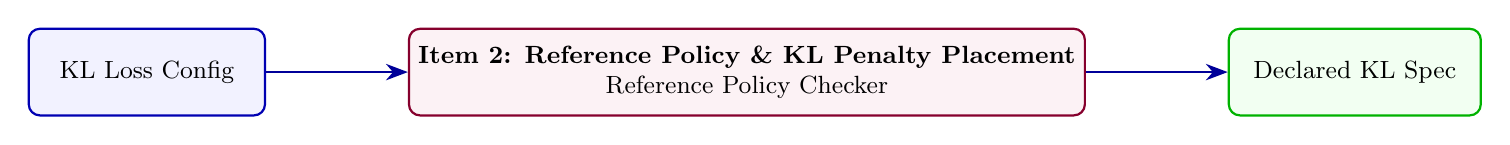
\begin{tikzpicture}[
    node distance=1.4cm and 1.8cm,
    box1/.style={rectangle, draw=blue!70!black, fill=blue!5, thick, rounded corners, align=center, minimum height=1.1cm, minimum width=3.0cm, font=\small},
    box2/.style={rectangle, draw=purple!70!black, fill=purple!5, thick, rounded corners, align=center, minimum height=1.1cm, minimum width=3.4cm, font=\small},
    box3/.style={rectangle, draw=green!70!black, fill=green!5, thick, rounded corners, align=center, minimum height=1.1cm, minimum width=3.2cm, font=\small},
    arrow/.style={-{Stealth[scale=1.2]}, thick, draw=blue!60!black}
]
    \node [box1] (n1) {KL Loss Config};
    \node [box2, right=of n1] (n2) {\textbf{Item 2: Reference Policy \& KL Penalty Placement}\\Reference Policy Checker};
    \node [box3, right=of n2] (n3) {Declared KL Spec};

    \draw [arrow] (n1) -- (n2);
    \draw [arrow] (n2) -- (n3);
\end{tikzpicture}
\caption{\textbf{Item 2: Reference Policy \& KL Penalty Placement}. Specification requirement for reference policy and KL terms.}
\label{fig:r06_item2_reference}
\end{figure}

\begin{figure}[htbp]
\centering
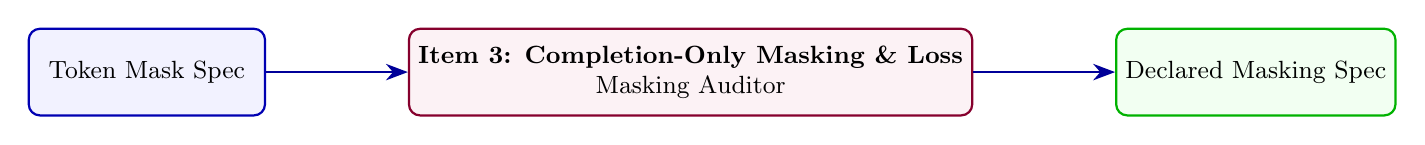
\begin{tikzpicture}[
    node distance=1.4cm and 1.8cm,
    box1/.style={rectangle, draw=blue!70!black, fill=blue!5, thick, rounded corners, align=center, minimum height=1.1cm, minimum width=3.0cm, font=\small},
    box2/.style={rectangle, draw=purple!70!black, fill=purple!5, thick, rounded corners, align=center, minimum height=1.1cm, minimum width=3.4cm, font=\small},
    box3/.style={rectangle, draw=green!70!black, fill=green!5, thick, rounded corners, align=center, minimum height=1.1cm, minimum width=3.2cm, font=\small},
    arrow/.style={-{Stealth[scale=1.2]}, thick, draw=blue!60!black}
]
    \node [box1] (n1) {Token Mask Spec};
    \node [box2, right=of n1] (n2) {\textbf{Item 3: Completion-Only Masking \& Loss}\\Masking Auditor};
    \node [box3, right=of n2] (n3) {Declared Masking Spec};

    \draw [arrow] (n1) -- (n2);
    \draw [arrow] (n2) -- (n3);
\end{tikzpicture}
\caption{\textbf{Item 3: Completion-Only Masking \& Loss}. Specification requirement for token loss masking rules.}
\label{fig:r06_item3_masking}
\end{figure}

\begin{figure}[htbp]
\centering
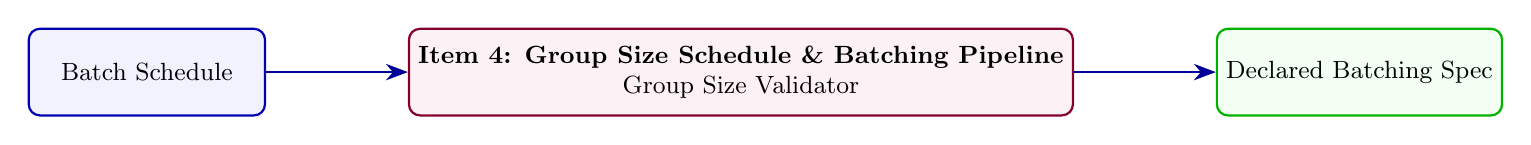
\begin{tikzpicture}[
    node distance=1.4cm and 1.8cm,
    box1/.style={rectangle, draw=blue!70!black, fill=blue!5, thick, rounded corners, align=center, minimum height=1.1cm, minimum width=3.0cm, font=\small},
    box2/.style={rectangle, draw=purple!70!black, fill=purple!5, thick, rounded corners, align=center, minimum height=1.1cm, minimum width=3.4cm, font=\small},
    box3/.style={rectangle, draw=green!70!black, fill=green!5, thick, rounded corners, align=center, minimum height=1.1cm, minimum width=3.2cm, font=\small},
    arrow/.style={-{Stealth[scale=1.2]}, thick, draw=blue!60!black}
]
    \node [box1] (n1) {Batch Schedule};
    \node [box2, right=of n1] (n2) {\textbf{Item 4: Group Size Schedule \& Batching Pipeline}\\Group Size Validator};
    \node [box3, right=of n2] (n3) {Declared Batching Spec};

    \draw [arrow] (n1) -- (n2);
    \draw [arrow] (n2) -- (n3);
\end{tikzpicture}
\caption{\textbf{Item 4: Group Size Schedule \& Batching Pipeline}. Specification requirement for group size and micro-batching.}
\label{fig:r06_item4_batching}
\end{figure}

\begin{figure}[htbp]
\centering
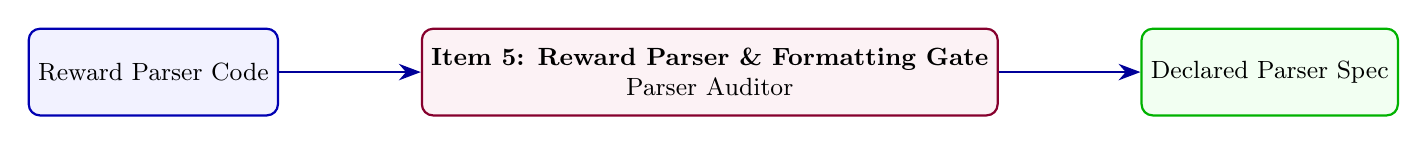
\begin{tikzpicture}[
    node distance=1.4cm and 1.8cm,
    box1/.style={rectangle, draw=blue!70!black, fill=blue!5, thick, rounded corners, align=center, minimum height=1.1cm, minimum width=3.0cm, font=\small},
    box2/.style={rectangle, draw=purple!70!black, fill=purple!5, thick, rounded corners, align=center, minimum height=1.1cm, minimum width=3.4cm, font=\small},
    box3/.style={rectangle, draw=green!70!black, fill=green!5, thick, rounded corners, align=center, minimum height=1.1cm, minimum width=3.2cm, font=\small},
    arrow/.style={-{Stealth[scale=1.2]}, thick, draw=blue!60!black}
]
    \node [box1] (n1) {Reward Parser Code};
    \node [box2, right=of n1] (n2) {\textbf{Item 5: Reward Parser \& Formatting Gate}\\Parser Auditor};
    \node [box3, right=of n2] (n3) {Declared Parser Spec};

    \draw [arrow] (n1) -- (n2);
    \draw [arrow] (n2) -- (n3);
\end{tikzpicture}
\caption{\textbf{Item 5: Reward Parser \& Formatting Gate}. Specification requirement for reward extraction rules.}
\label{fig:r06_item5_parser}
\end{figure}

\begin{figure}[htbp]
\centering
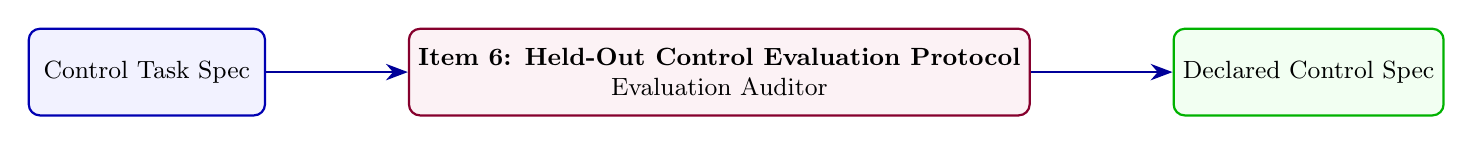
\begin{tikzpicture}[
    node distance=1.4cm and 1.8cm,
    box1/.style={rectangle, draw=blue!70!black, fill=blue!5, thick, rounded corners, align=center, minimum height=1.1cm, minimum width=3.0cm, font=\small},
    box2/.style={rectangle, draw=purple!70!black, fill=purple!5, thick, rounded corners, align=center, minimum height=1.1cm, minimum width=3.4cm, font=\small},
    box3/.style={rectangle, draw=green!70!black, fill=green!5, thick, rounded corners, align=center, minimum height=1.1cm, minimum width=3.2cm, font=\small},
    arrow/.style={-{Stealth[scale=1.2]}, thick, draw=blue!60!black}
]
    \node [box1] (n1) {Control Task Spec};
    \node [box2, right=of n1] (n2) {\textbf{Item 6: Held-Out Control Evaluation Protocol}\\Evaluation Auditor};
    \node [box3, right=of n2] (n3) {Declared Control Spec};

    \draw [arrow] (n1) -- (n2);
    \draw [arrow] (n2) -- (n3);
\end{tikzpicture}
\caption{\textbf{Item 6: Held-Out Control Evaluation Protocol}. Specification requirement for held-out task evaluation.}
\label{fig:r06_item6_eval}
\end{figure}

\begin{figure}[htbp]
\centering
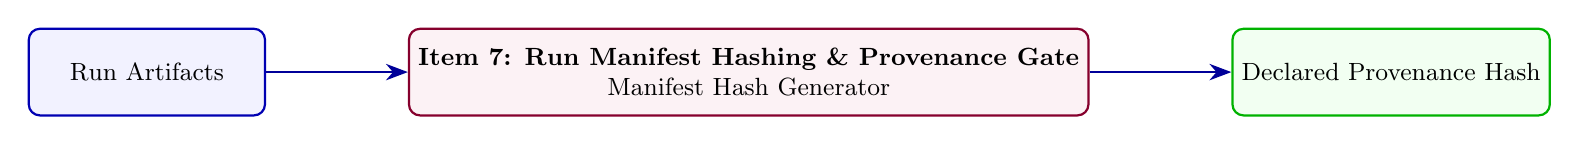
\begin{tikzpicture}[
    node distance=1.4cm and 1.8cm,
    box1/.style={rectangle, draw=blue!70!black, fill=blue!5, thick, rounded corners, align=center, minimum height=1.1cm, minimum width=3.0cm, font=\small},
    box2/.style={rectangle, draw=purple!70!black, fill=purple!5, thick, rounded corners, align=center, minimum height=1.1cm, minimum width=3.4cm, font=\small},
    box3/.style={rectangle, draw=green!70!black, fill=green!5, thick, rounded corners, align=center, minimum height=1.1cm, minimum width=3.2cm, font=\small},
    arrow/.style={-{Stealth[scale=1.2]}, thick, draw=blue!60!black}
]
    \node [box1] (n1) {Run Artifacts};
    \node [box2, right=of n1] (n2) {\textbf{Item 7: Run Manifest Hashing \& Provenance Gate}\\Manifest Hash Generator};
    \node [box3, right=of n2] (n3) {Declared Provenance Hash};

    \draw [arrow] (n1) -- (n2);
    \draw [arrow] (n2) -- (n3);
\end{tikzpicture}
\caption{\textbf{Item 7: Run Manifest Hashing \& Provenance Gate}. Specification requirement for cryptographic run hashing.}
\label{fig:r06_item7_manifest}
\end{figure}

\begin{figure}[htbp]
\centering
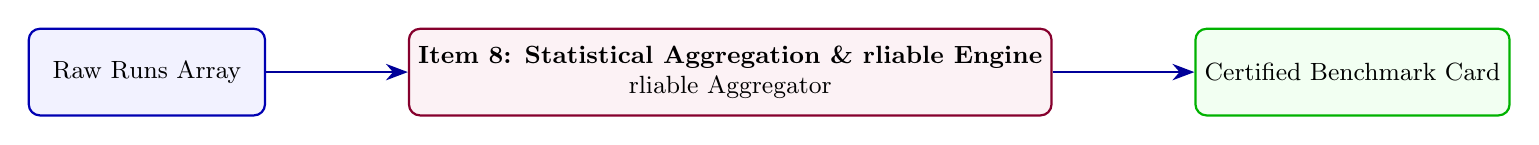
\begin{tikzpicture}[
    node distance=1.4cm and 1.8cm,
    box1/.style={rectangle, draw=blue!70!black, fill=blue!5, thick, rounded corners, align=center, minimum height=1.1cm, minimum width=3.0cm, font=\small},
    box2/.style={rectangle, draw=purple!70!black, fill=purple!5, thick, rounded corners, align=center, minimum height=1.1cm, minimum width=3.4cm, font=\small},
    box3/.style={rectangle, draw=green!70!black, fill=green!5, thick, rounded corners, align=center, minimum height=1.1cm, minimum width=3.2cm, font=\small},
    arrow/.style={-{Stealth[scale=1.2]}, thick, draw=blue!60!black}
]
    \node [box1] (n1) {Raw Runs Array};
    \node [box2, right=of n1] (n2) {\textbf{Item 8: Statistical Aggregation \& rliable Engine}\\rliable Aggregator};
    \node [box3, right=of n2] (n3) {Certified Benchmark Card};

    \draw [arrow] (n1) -- (n2);
    \draw [arrow] (n2) -- (n3);
\end{tikzpicture}
\caption{\textbf{Item 8: Statistical Aggregation \& rliable Engine}. Specification requirement for statistical performance profiles.}
\label{fig:r06_item8_aggregation}
\end{figure}



\begin{figure}[htbp]
\centering
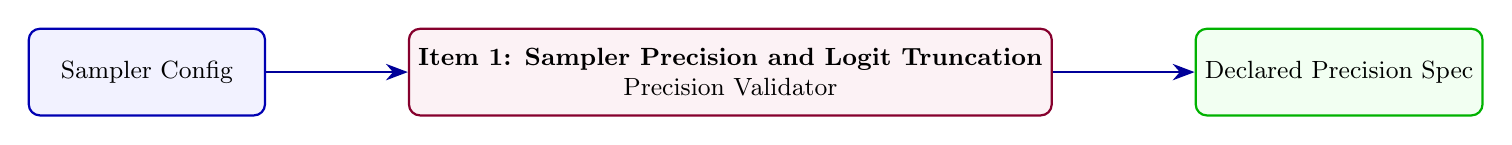
\begin{tikzpicture}[
    node distance=1.4cm and 1.8cm,
    b1/.style={rectangle, draw=blue!70!black, fill=blue!5, thick, rounded corners, align=center, minimum height=1.1cm, minimum width=3.0cm, font=\small},
    b2/.style={rectangle, draw=purple!70!black, fill=purple!5, thick, rounded corners, align=center, minimum height=1.1cm, minimum width=3.4cm, font=\small},
    b3/.style={rectangle, draw=green!70!black, fill=green!5, thick, rounded corners, align=center, minimum height=1.1cm, minimum width=3.2cm, font=\small},
    arr/.style={-{Stealth[scale=1.2]}, thick, draw=blue!60!black}
]
    \node [b1] (n1) {Sampler Config};
    \node [b2, right=of n1] (n2) {\textbf{Item 1: Sampler Precision and Logit Truncation}\\Precision Validator};
    \node [b3, right=of n2] (n3) {Declared Precision Spec};

    \draw [arr] (n1) -- (n2);
    \draw [arr] (n2) -- (n3);
\end{tikzpicture}
\caption{\textbf{Item 1: Sampler Precision and Logit Truncation}. Specification requirement for floating-point sampler precision.}
\label{fig:r06_fig1}
\end{figure}

\begin{figure}[htbp]
\centering
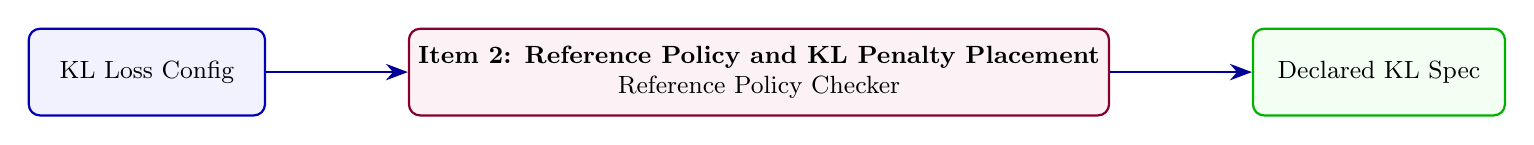
\begin{tikzpicture}[
    node distance=1.4cm and 1.8cm,
    b1/.style={rectangle, draw=blue!70!black, fill=blue!5, thick, rounded corners, align=center, minimum height=1.1cm, minimum width=3.0cm, font=\small},
    b2/.style={rectangle, draw=purple!70!black, fill=purple!5, thick, rounded corners, align=center, minimum height=1.1cm, minimum width=3.4cm, font=\small},
    b3/.style={rectangle, draw=green!70!black, fill=green!5, thick, rounded corners, align=center, minimum height=1.1cm, minimum width=3.2cm, font=\small},
    arr/.style={-{Stealth[scale=1.2]}, thick, draw=blue!60!black}
]
    \node [b1] (n1) {KL Loss Config};
    \node [b2, right=of n1] (n2) {\textbf{Item 2: Reference Policy and KL Penalty Placement}\\Reference Policy Checker};
    \node [b3, right=of n2] (n3) {Declared KL Spec};

    \draw [arr] (n1) -- (n2);
    \draw [arr] (n2) -- (n3);
\end{tikzpicture}
\caption{\textbf{Item 2: Reference Policy and KL Penalty Placement}. Specification requirement for reference policy and KL terms.}
\label{fig:r06_fig2}
\end{figure}

\begin{figure}[htbp]
\centering
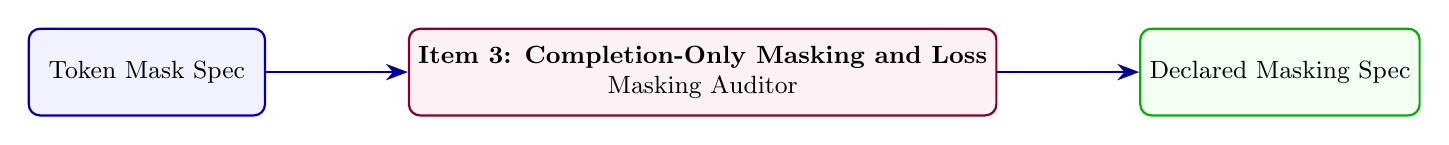
\begin{tikzpicture}[
    node distance=1.4cm and 1.8cm,
    b1/.style={rectangle, draw=blue!70!black, fill=blue!5, thick, rounded corners, align=center, minimum height=1.1cm, minimum width=3.0cm, font=\small},
    b2/.style={rectangle, draw=purple!70!black, fill=purple!5, thick, rounded corners, align=center, minimum height=1.1cm, minimum width=3.4cm, font=\small},
    b3/.style={rectangle, draw=green!70!black, fill=green!5, thick, rounded corners, align=center, minimum height=1.1cm, minimum width=3.2cm, font=\small},
    arr/.style={-{Stealth[scale=1.2]}, thick, draw=blue!60!black}
]
    \node [b1] (n1) {Token Mask Spec};
    \node [b2, right=of n1] (n2) {\textbf{Item 3: Completion-Only Masking and Loss}\\Masking Auditor};
    \node [b3, right=of n2] (n3) {Declared Masking Spec};

    \draw [arr] (n1) -- (n2);
    \draw [arr] (n2) -- (n3);
\end{tikzpicture}
\caption{\textbf{Item 3: Completion-Only Masking and Loss}. Specification requirement for token loss masking rules.}
\label{fig:r06_fig3}
\end{figure}

\begin{figure}[htbp]
\centering
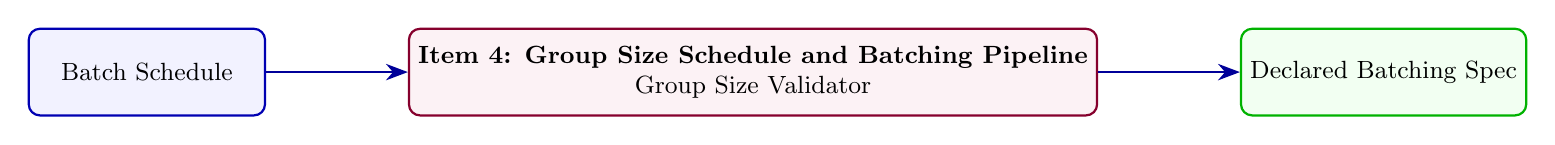
\begin{tikzpicture}[
    node distance=1.4cm and 1.8cm,
    b1/.style={rectangle, draw=blue!70!black, fill=blue!5, thick, rounded corners, align=center, minimum height=1.1cm, minimum width=3.0cm, font=\small},
    b2/.style={rectangle, draw=purple!70!black, fill=purple!5, thick, rounded corners, align=center, minimum height=1.1cm, minimum width=3.4cm, font=\small},
    b3/.style={rectangle, draw=green!70!black, fill=green!5, thick, rounded corners, align=center, minimum height=1.1cm, minimum width=3.2cm, font=\small},
    arr/.style={-{Stealth[scale=1.2]}, thick, draw=blue!60!black}
]
    \node [b1] (n1) {Batch Schedule};
    \node [b2, right=of n1] (n2) {\textbf{Item 4: Group Size Schedule and Batching Pipeline}\\Group Size Validator};
    \node [b3, right=of n2] (n3) {Declared Batching Spec};

    \draw [arr] (n1) -- (n2);
    \draw [arr] (n2) -- (n3);
\end{tikzpicture}
\caption{\textbf{Item 4: Group Size Schedule and Batching Pipeline}. Specification requirement for group size and micro-batching.}
\label{fig:r06_fig4}
\end{figure}

\begin{figure}[htbp]
\centering
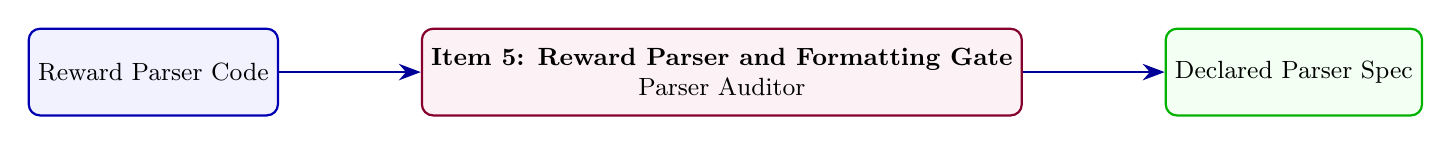
\begin{tikzpicture}[
    node distance=1.4cm and 1.8cm,
    b1/.style={rectangle, draw=blue!70!black, fill=blue!5, thick, rounded corners, align=center, minimum height=1.1cm, minimum width=3.0cm, font=\small},
    b2/.style={rectangle, draw=purple!70!black, fill=purple!5, thick, rounded corners, align=center, minimum height=1.1cm, minimum width=3.4cm, font=\small},
    b3/.style={rectangle, draw=green!70!black, fill=green!5, thick, rounded corners, align=center, minimum height=1.1cm, minimum width=3.2cm, font=\small},
    arr/.style={-{Stealth[scale=1.2]}, thick, draw=blue!60!black}
]
    \node [b1] (n1) {Reward Parser Code};
    \node [b2, right=of n1] (n2) {\textbf{Item 5: Reward Parser and Formatting Gate}\\Parser Auditor};
    \node [b3, right=of n2] (n3) {Declared Parser Spec};

    \draw [arr] (n1) -- (n2);
    \draw [arr] (n2) -- (n3);
\end{tikzpicture}
\caption{\textbf{Item 5: Reward Parser and Formatting Gate}. Specification requirement for reward extraction rules.}
\label{fig:r06_fig5}
\end{figure}

\begin{figure}[htbp]
\centering
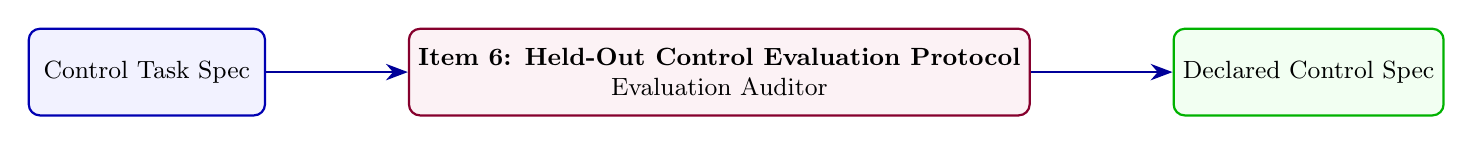
\begin{tikzpicture}[
    node distance=1.4cm and 1.8cm,
    b1/.style={rectangle, draw=blue!70!black, fill=blue!5, thick, rounded corners, align=center, minimum height=1.1cm, minimum width=3.0cm, font=\small},
    b2/.style={rectangle, draw=purple!70!black, fill=purple!5, thick, rounded corners, align=center, minimum height=1.1cm, minimum width=3.4cm, font=\small},
    b3/.style={rectangle, draw=green!70!black, fill=green!5, thick, rounded corners, align=center, minimum height=1.1cm, minimum width=3.2cm, font=\small},
    arr/.style={-{Stealth[scale=1.2]}, thick, draw=blue!60!black}
]
    \node [b1] (n1) {Control Task Spec};
    \node [b2, right=of n1] (n2) {\textbf{Item 6: Held-Out Control Evaluation Protocol}\\Evaluation Auditor};
    \node [b3, right=of n2] (n3) {Declared Control Spec};

    \draw [arr] (n1) -- (n2);
    \draw [arr] (n2) -- (n3);
\end{tikzpicture}
\caption{\textbf{Item 6: Held-Out Control Evaluation Protocol}. Specification requirement for held-out task evaluation.}
\label{fig:r06_fig6}
\end{figure}

\begin{figure}[htbp]
\centering
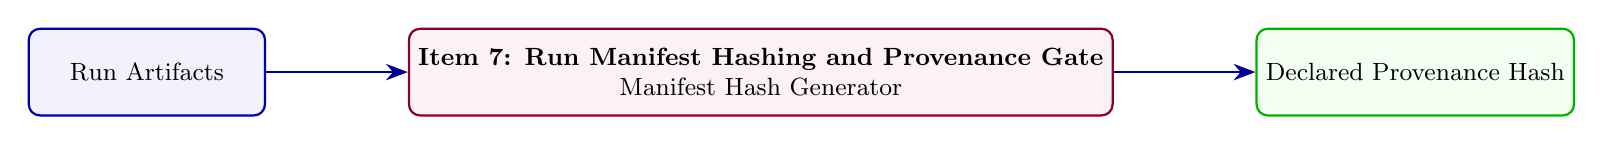
\begin{tikzpicture}[
    node distance=1.4cm and 1.8cm,
    b1/.style={rectangle, draw=blue!70!black, fill=blue!5, thick, rounded corners, align=center, minimum height=1.1cm, minimum width=3.0cm, font=\small},
    b2/.style={rectangle, draw=purple!70!black, fill=purple!5, thick, rounded corners, align=center, minimum height=1.1cm, minimum width=3.4cm, font=\small},
    b3/.style={rectangle, draw=green!70!black, fill=green!5, thick, rounded corners, align=center, minimum height=1.1cm, minimum width=3.2cm, font=\small},
    arr/.style={-{Stealth[scale=1.2]}, thick, draw=blue!60!black}
]
    \node [b1] (n1) {Run Artifacts};
    \node [b2, right=of n1] (n2) {\textbf{Item 7: Run Manifest Hashing and Provenance Gate}\\Manifest Hash Generator};
    \node [b3, right=of n2] (n3) {Declared Provenance Hash};

    \draw [arr] (n1) -- (n2);
    \draw [arr] (n2) -- (n3);
\end{tikzpicture}
\caption{\textbf{Item 7: Run Manifest Hashing and Provenance Gate}. Specification requirement for cryptographic run hashing.}
\label{fig:r06_fig7}
\end{figure}

\begin{figure}[htbp]
\centering
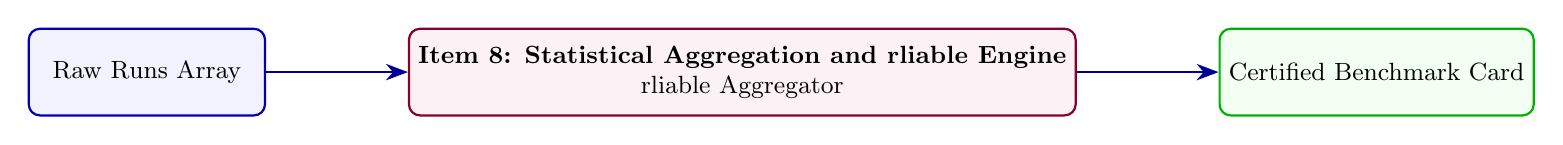
\begin{tikzpicture}[
    node distance=1.4cm and 1.8cm,
    b1/.style={rectangle, draw=blue!70!black, fill=blue!5, thick, rounded corners, align=center, minimum height=1.1cm, minimum width=3.0cm, font=\small},
    b2/.style={rectangle, draw=purple!70!black, fill=purple!5, thick, rounded corners, align=center, minimum height=1.1cm, minimum width=3.4cm, font=\small},
    b3/.style={rectangle, draw=green!70!black, fill=green!5, thick, rounded corners, align=center, minimum height=1.1cm, minimum width=3.2cm, font=\small},
    arr/.style={-{Stealth[scale=1.2]}, thick, draw=blue!60!black}
]
    \node [b1] (n1) {Raw Runs Array};
    \node [b2, right=of n1] (n2) {\textbf{Item 8: Statistical Aggregation and rliable Engine}\\rliable Aggregator};
    \node [b3, right=of n2] (n3) {Certified Benchmark Card};

    \draw [arr] (n1) -- (n2);
    \draw [arr] (n2) -- (n3);
\end{tikzpicture}
\caption{\textbf{Item 8: Statistical Aggregation and rliable Engine}. Specification requirement for statistical performance profiles.}
\label{fig:r06_fig8}
\end{figure}



\begin{figure}[htbp]
\centering
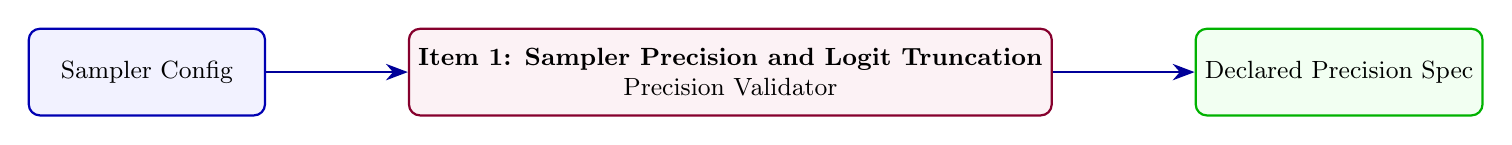
\begin{tikzpicture}[
    node distance=1.4cm and 1.8cm,
    b1/.style={rectangle, draw=blue!70!black, fill=blue!5, thick, rounded corners, align=center, minimum height=1.1cm, minimum width=3.0cm, font=\small},
    b2/.style={rectangle, draw=purple!70!black, fill=purple!5, thick, rounded corners, align=center, minimum height=1.1cm, minimum width=3.4cm, font=\small},
    b3/.style={rectangle, draw=green!70!black, fill=green!5, thick, rounded corners, align=center, minimum height=1.1cm, minimum width=3.2cm, font=\small},
    arr/.style={-{Stealth[scale=1.2]}, thick, draw=blue!60!black}
]
    \node [b1] (n1) {Sampler Config};
    \node [b2, right=of n1] (n2) {\textbf{Item 1: Sampler Precision and Logit Truncation}\\Precision Validator};
    \node [b3, right=of n2] (n3) {Declared Precision Spec};

    \draw [arr] (n1) -- (n2);
    \draw [arr] (n2) -- (n3);
\end{tikzpicture}
\caption{\textbf{Item 1: Sampler Precision and Logit Truncation}. Specification requirement for floating-point sampler precision.}
\label{fig:r06_fig1}
\end{figure}

\begin{figure}[htbp]
\centering
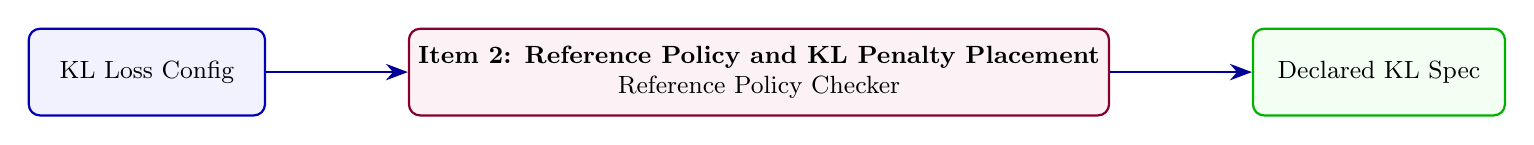
\begin{tikzpicture}[
    node distance=1.4cm and 1.8cm,
    b1/.style={rectangle, draw=blue!70!black, fill=blue!5, thick, rounded corners, align=center, minimum height=1.1cm, minimum width=3.0cm, font=\small},
    b2/.style={rectangle, draw=purple!70!black, fill=purple!5, thick, rounded corners, align=center, minimum height=1.1cm, minimum width=3.4cm, font=\small},
    b3/.style={rectangle, draw=green!70!black, fill=green!5, thick, rounded corners, align=center, minimum height=1.1cm, minimum width=3.2cm, font=\small},
    arr/.style={-{Stealth[scale=1.2]}, thick, draw=blue!60!black}
]
    \node [b1] (n1) {KL Loss Config};
    \node [b2, right=of n1] (n2) {\textbf{Item 2: Reference Policy and KL Penalty Placement}\\Reference Policy Checker};
    \node [b3, right=of n2] (n3) {Declared KL Spec};

    \draw [arr] (n1) -- (n2);
    \draw [arr] (n2) -- (n3);
\end{tikzpicture}
\caption{\textbf{Item 2: Reference Policy and KL Penalty Placement}. Specification requirement for reference policy and KL terms.}
\label{fig:r06_fig2}
\end{figure}

\begin{figure}[htbp]
\centering
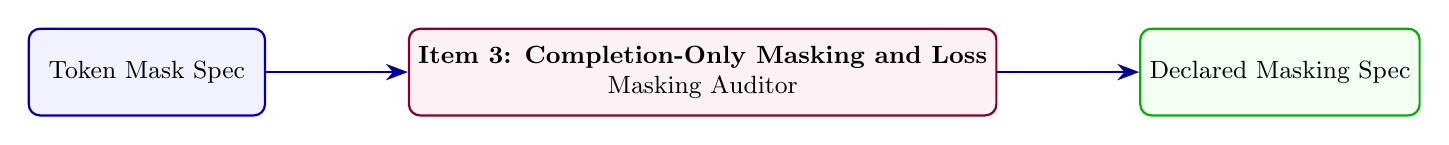
\begin{tikzpicture}[
    node distance=1.4cm and 1.8cm,
    b1/.style={rectangle, draw=blue!70!black, fill=blue!5, thick, rounded corners, align=center, minimum height=1.1cm, minimum width=3.0cm, font=\small},
    b2/.style={rectangle, draw=purple!70!black, fill=purple!5, thick, rounded corners, align=center, minimum height=1.1cm, minimum width=3.4cm, font=\small},
    b3/.style={rectangle, draw=green!70!black, fill=green!5, thick, rounded corners, align=center, minimum height=1.1cm, minimum width=3.2cm, font=\small},
    arr/.style={-{Stealth[scale=1.2]}, thick, draw=blue!60!black}
]
    \node [b1] (n1) {Token Mask Spec};
    \node [b2, right=of n1] (n2) {\textbf{Item 3: Completion-Only Masking and Loss}\\Masking Auditor};
    \node [b3, right=of n2] (n3) {Declared Masking Spec};

    \draw [arr] (n1) -- (n2);
    \draw [arr] (n2) -- (n3);
\end{tikzpicture}
\caption{\textbf{Item 3: Completion-Only Masking and Loss}. Specification requirement for token loss masking rules.}
\label{fig:r06_fig3}
\end{figure}

\begin{figure}[htbp]
\centering
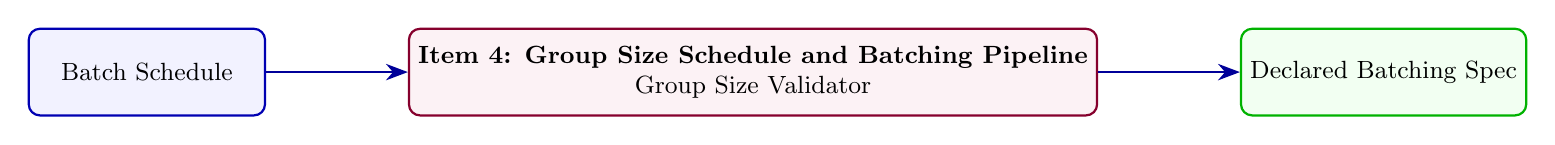
\begin{tikzpicture}[
    node distance=1.4cm and 1.8cm,
    b1/.style={rectangle, draw=blue!70!black, fill=blue!5, thick, rounded corners, align=center, minimum height=1.1cm, minimum width=3.0cm, font=\small},
    b2/.style={rectangle, draw=purple!70!black, fill=purple!5, thick, rounded corners, align=center, minimum height=1.1cm, minimum width=3.4cm, font=\small},
    b3/.style={rectangle, draw=green!70!black, fill=green!5, thick, rounded corners, align=center, minimum height=1.1cm, minimum width=3.2cm, font=\small},
    arr/.style={-{Stealth[scale=1.2]}, thick, draw=blue!60!black}
]
    \node [b1] (n1) {Batch Schedule};
    \node [b2, right=of n1] (n2) {\textbf{Item 4: Group Size Schedule and Batching Pipeline}\\Group Size Validator};
    \node [b3, right=of n2] (n3) {Declared Batching Spec};

    \draw [arr] (n1) -- (n2);
    \draw [arr] (n2) -- (n3);
\end{tikzpicture}
\caption{\textbf{Item 4: Group Size Schedule and Batching Pipeline}. Specification requirement for group size and micro-batching.}
\label{fig:r06_fig4}
\end{figure}

\begin{figure}[htbp]
\centering
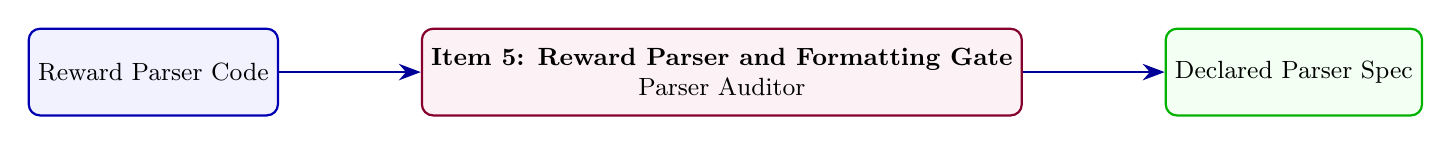
\begin{tikzpicture}[
    node distance=1.4cm and 1.8cm,
    b1/.style={rectangle, draw=blue!70!black, fill=blue!5, thick, rounded corners, align=center, minimum height=1.1cm, minimum width=3.0cm, font=\small},
    b2/.style={rectangle, draw=purple!70!black, fill=purple!5, thick, rounded corners, align=center, minimum height=1.1cm, minimum width=3.4cm, font=\small},
    b3/.style={rectangle, draw=green!70!black, fill=green!5, thick, rounded corners, align=center, minimum height=1.1cm, minimum width=3.2cm, font=\small},
    arr/.style={-{Stealth[scale=1.2]}, thick, draw=blue!60!black}
]
    \node [b1] (n1) {Reward Parser Code};
    \node [b2, right=of n1] (n2) {\textbf{Item 5: Reward Parser and Formatting Gate}\\Parser Auditor};
    \node [b3, right=of n2] (n3) {Declared Parser Spec};

    \draw [arr] (n1) -- (n2);
    \draw [arr] (n2) -- (n3);
\end{tikzpicture}
\caption{\textbf{Item 5: Reward Parser and Formatting Gate}. Specification requirement for reward extraction rules.}
\label{fig:r06_fig5}
\end{figure}

\begin{figure}[htbp]
\centering
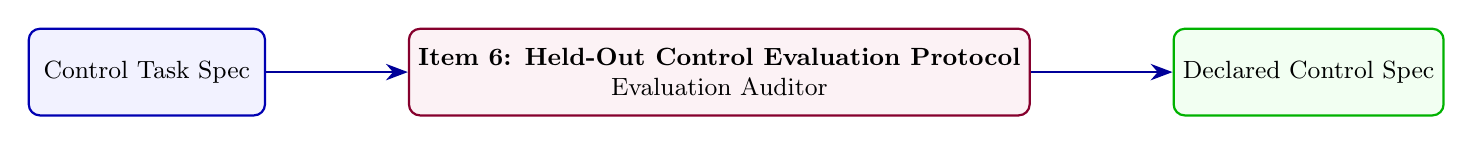
\begin{tikzpicture}[
    node distance=1.4cm and 1.8cm,
    b1/.style={rectangle, draw=blue!70!black, fill=blue!5, thick, rounded corners, align=center, minimum height=1.1cm, minimum width=3.0cm, font=\small},
    b2/.style={rectangle, draw=purple!70!black, fill=purple!5, thick, rounded corners, align=center, minimum height=1.1cm, minimum width=3.4cm, font=\small},
    b3/.style={rectangle, draw=green!70!black, fill=green!5, thick, rounded corners, align=center, minimum height=1.1cm, minimum width=3.2cm, font=\small},
    arr/.style={-{Stealth[scale=1.2]}, thick, draw=blue!60!black}
]
    \node [b1] (n1) {Control Task Spec};
    \node [b2, right=of n1] (n2) {\textbf{Item 6: Held-Out Control Evaluation Protocol}\\Evaluation Auditor};
    \node [b3, right=of n2] (n3) {Declared Control Spec};

    \draw [arr] (n1) -- (n2);
    \draw [arr] (n2) -- (n3);
\end{tikzpicture}
\caption{\textbf{Item 6: Held-Out Control Evaluation Protocol}. Specification requirement for held-out task evaluation.}
\label{fig:r06_fig6}
\end{figure}

\begin{figure}[htbp]
\centering
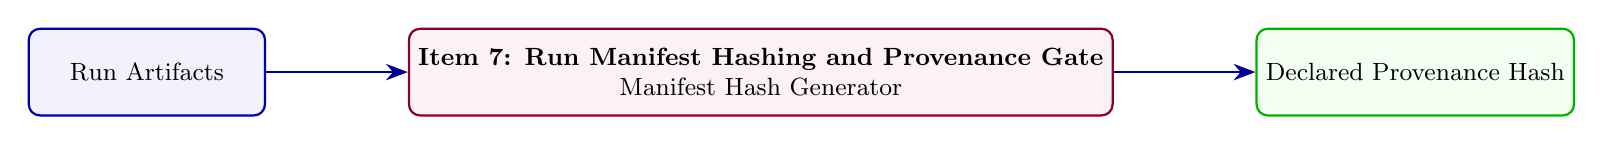
\begin{tikzpicture}[
    node distance=1.4cm and 1.8cm,
    b1/.style={rectangle, draw=blue!70!black, fill=blue!5, thick, rounded corners, align=center, minimum height=1.1cm, minimum width=3.0cm, font=\small},
    b2/.style={rectangle, draw=purple!70!black, fill=purple!5, thick, rounded corners, align=center, minimum height=1.1cm, minimum width=3.4cm, font=\small},
    b3/.style={rectangle, draw=green!70!black, fill=green!5, thick, rounded corners, align=center, minimum height=1.1cm, minimum width=3.2cm, font=\small},
    arr/.style={-{Stealth[scale=1.2]}, thick, draw=blue!60!black}
]
    \node [b1] (n1) {Run Artifacts};
    \node [b2, right=of n1] (n2) {\textbf{Item 7: Run Manifest Hashing and Provenance Gate}\\Manifest Hash Generator};
    \node [b3, right=of n2] (n3) {Declared Provenance Hash};

    \draw [arr] (n1) -- (n2);
    \draw [arr] (n2) -- (n3);
\end{tikzpicture}
\caption{\textbf{Item 7: Run Manifest Hashing and Provenance Gate}. Specification requirement for cryptographic run hashing.}
\label{fig:r06_fig7}
\end{figure}

\begin{figure}[htbp]
\centering
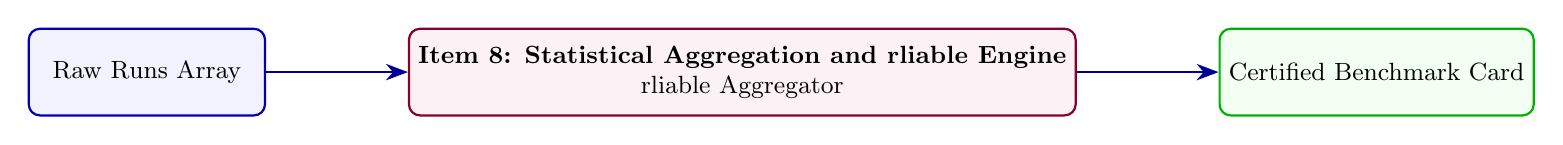
\begin{tikzpicture}[
    node distance=1.4cm and 1.8cm,
    b1/.style={rectangle, draw=blue!70!black, fill=blue!5, thick, rounded corners, align=center, minimum height=1.1cm, minimum width=3.0cm, font=\small},
    b2/.style={rectangle, draw=purple!70!black, fill=purple!5, thick, rounded corners, align=center, minimum height=1.1cm, minimum width=3.4cm, font=\small},
    b3/.style={rectangle, draw=green!70!black, fill=green!5, thick, rounded corners, align=center, minimum height=1.1cm, minimum width=3.2cm, font=\small},
    arr/.style={-{Stealth[scale=1.2]}, thick, draw=blue!60!black}
]
    \node [b1] (n1) {Raw Runs Array};
    \node [b2, right=of n1] (n2) {\textbf{Item 8: Statistical Aggregation and rliable Engine}\\rliable Aggregator};
    \node [b3, right=of n2] (n3) {Certified Benchmark Card};

    \draw [arr] (n1) -- (n2);
    \draw [arr] (n2) -- (n3);
\end{tikzpicture}
\caption{\textbf{Item 8: Statistical Aggregation and rliable Engine}. Specification requirement for statistical performance profiles.}
\label{fig:r06_fig8}
\end{figure}

\end{document}
